\documentclass[italian,master]{unibg}

\usepackage{color}
\usepackage{amsmath}
\usepackage{titlesec}
\usepackage{subcaption}

\newcommand{\todo}[1]{{\color{red} TODO: #1}}

% ==== FRONTESPIZIO ====
\title{Produzione scientifica}
\subtitle{Analisi e confronto delle principali metriche di valutazione}
\advisor{Chiar.mo Prof.~Stefano Paraboschi}

\department{Ingegneria Gestionale, dell'Informazione e della Produzione}
\course{Ingegneria Informatica}
\class{LM-32}

\author{Bianca Crippa}
\studentid{1053356}
\year{2022/2023}

% ==== FANCY TITLES ====
\definecolor{gray75}{gray}{0.75}
\newcommand{\PRLsep}{\noindent\makebox[\linewidth]{\resizebox{\linewidth}{1.5pt}{\textcolor{gray75}{$\bullet$}}}}
\renewcommand{\headrulewidth}{0pt}
\titleformat{\chapter}[hang]{\centering\Huge\bfseries}{\thechapter.\hspace{10pt}}{0pt}{\Huge\bfseries}[\vspace*{-0.7\baselineskip}\PRLsep]

% ==== CODE SYNTAX HIGHLIGHTING ====

\definecolor{codegreen}{rgb}{0,0.6,0}
\definecolor{codegray}{rgb}{0.5,0.5,0.5}
\definecolor{codeblue}{rgb}{0,0,1}
\definecolor{backcolour}{rgb}{0.95,0.95,0.92}

\lstset{
    backgroundcolor=\color{backcolour},   
    commentstyle=\color{codegreen},
    keywordstyle=\color{magenta},
    numberstyle=\tiny\color{codegray},
    stringstyle=\color{codeblue},
    basicstyle=\ttfamily\footnotesize,
    breakatwhitespace=false,         
    breaklines=true,                 
    captionpos=b,                    
    keepspaces=true,                 
    numbers=left,                    
    numbersep=5pt,                  
    showspaces=false,                
    showstringspaces=false,
    showtabs=false,                  
    tabsize=2,
    upquote=true,
    float=tb,
}
% Workaround to make all listings float by default
% https://tex.stackexchange.com/questions/128713/lstinputlisting-does-not-respect-the-lstset-float-option
\makeatletter
\let\lst@floatdefault\lst@float
\makeatother

\begin{document}
\renewcommand{\abstractname}{Abstract}
\maketitle
\emptypage
\begin{abstract}

Questo progetto di tesi consiste in un'analisi di dati riguardanti la valutazione della produzione scientifica.

Sono state prodotte delle metriche per affiliazioni, autori e conferenze, mostrando il forte impatto che conferenze di livello top e grandi affiliazioni hanno su parametri come l'$h$-index di un autore o il numero di citazioni di un paper. 

\end{abstract}
\emptypage
\toc[figures,tables,listings]
% \emptypage

\clearpage
\pagenumbering{arabic}

\chapter{Introduzione}

%%%%%% OBIETTIVI %%%%%%%%
\section{Obiettivi del progetto}

Questo progetto di tesi si pone l’obiettivo di trovare delle relazioni tra
diversi indici bibliometrici che vengono utilizzati  per valutare la produzione
accademica. Una visione complessiva dei dati può essere utile per valutare gli
andamenti e migliorare la produttività accademica. L’applicazione sviluppata
permette, tramite interfaccia grafica, di gestire e visualizzare autori, paper,
università e conferenze, interfacciandosi con un database per l’inserimento e
l’interrogazione dei dati.

L'analisi di tali indici si concentra principalmente su quelli derivati da conferenze,
descritte in Sezione~\ref{sec:conferenze}.

%%%%%% CONTESTO %%%%%%%%%

\section{Contesto}


Nell’ambito della pubblicazione di testi di interesse accademico, una
\textit{pubblicazione scientifica} è definita come uno scritto oggettivo
riguardante un argomento scientifico, redatto da ricercatori o gruppi di ricerca
universitari.

Il gruppo di ricerca rende ufficialmente pubblici i metodi e i risultati delle
proprie ricerche sottoponendo il paper ad una conferenza oppure pubblicandolo
su riviste accademiche. Le pubblicazioni sono regolamentate da procedure di
accettazione e valutazione per stabilire se il lavoro presentato possieda i
requisiti per essere pubblicato.

\subsection{Criteri e classificazioni di pubblicazioni scientifiche}

Le pubblicazioni scientifiche vengono suddivise dal Ministero dell'Istruzione,
dell'Università e della Ricerca in una serie di categorie
\cite{criteri2009pubblicazioni}, che sono:

\begin{itemize}
    \item Gli \textit{articoli pubblicati su riviste scientifiche}, che
    riportano un codice ISSN e che sono stati  sottoposti a una procedura di
    revisione prima della pubblicazione per garantire autorevolezza;
    \item Le \textit{monografie di ricerca} che riportano codice ISBN e hanno
    superato la procedura di  accettazione per la pubblicazione;
    \item Gli \textit{articoli pubblicati in volumi collettivi}, sottoposti
    anch'essi alle stesse procedure di  accettazione degli articoli pubblicati
    su riviste scientifiche;
    \item Tutto ciò che sia riconducibile ad attività di ricerca, come brevetti, software, disegni, 
    purché accompagnati da pubblicazioni e documentazione per poter essere valutati.
\end{itemize}
%
Questi non risultano essere però l'unica classificazione esistente. Un altro
esempio di classificazione, seppur molto simile, è visibile in~\cite{oechsner2013}.

Inoltre, il MIUR ha anche proposto quattro criteri che devono essere
simultaneamente soddisfatti affinché un certo documento possa essere definito
come ``pubblicazione accademica'' \cite{criteri2013pubblicazioni}.
Essi sono:

\begin{itemize}
    \item I risultati presentati devono essere originali;
    \item I risultati presentati devono poter essere verificati e riutilizzati
    in altre attività di ricerca;
    \item Il linguaggio deve rendere la pubblicazione accessibile alla maggior
    parte delle persone interessate;
    \item La sede editoriale deve assicurare l’esistenza di una \textit{peer review} esterna.
\end{itemize}

Oltre a tali criteri, considerati di carattere generale, lo stesso
documento~\cite{criteri2013pubblicazioni} propone altri proprietà specifiche per
pubblicazioni e riviste scientifiche.

In particolare, una \textit{pubblicazione} può considerarsi scientifica se
espone in modo sistematico i risultati originali del lavoro di ricerca facendo
uso di riferimenti bibliografici, in modo tale che possano essere verificati da
terzi e riutilizzati in altre attività di ricerca.
Dev'essere inoltre sottoposta ad una procedura di revisione ed essere disponibile
in biblioteche universitarie o pubblicamente.

Diversamente, una \textit{rivista} è considerata scientifica se aderisce ai criteri
generali elencati prima, la revisione è formalizzata ed anonima, e garantisce una
periodicità nelle sue uscite.

\subsection{Struttura di una pubblicazione}

Una pubblicazione deve necessariamente presentare i seguenti campi:
\begin{itemize}
    \item \textit{Titolo}: deve fornire un riassunto di ciò che viene trattato
    nell'articolo;
    \item \textit{Nomi degli autori}: solitamente viene elencato seguendo
    l'ordine alfabetico oppure indicando il nome del ricercatore che ha
    contribuito maggiormente alla ricerca;
    \item \textit{Abstract}: un sommario per descrivere gli aspetti fondamentali
    del lavoro;
    \item \textit{Parole chiave}: lista di parole che si riferiscono agli
    argomenti trattati nell'articolo;
    \item \textit{Classificazione tematica};
    \item \textit{Introduzione}: breve paragrafo che indica gli scopi della ricerca;
    \item \textit{Metodi}: modi in cui sono stati condotti gli studi, i quali
    è fondamentale che usino procedure scientifiche, riproducibili da chiunque
    e confutabili;
    \item \textit{Risultati}: elenco dei dati scientifici ottenuti;
    \item \textit{Discussione}: interpretazione e analisi oggettiva dei dati;
    \item \textit{Conclusione}: considerazioni ed epilogo del lavoro svolto;
    \item \textit{Riferimenti}: elenco delle note bibliografiche;
    \item \textit{Riconoscimenti, appendici e supplementi}: informazioni accessorie.
\end{itemize}

\subsection{Conferenze scientifiche}\label{sec:conferenze}
\label{sec:conferenze_scientifiche}

Una conferenza scientifica è un evento al quale i ricercatori prendono parte per presentare e discurere i propri lavori accademici. Le conferenze sono un modo per scambiarsi informazioni, ricevere feedback da altri ricercatori, stabilire nuovi contatti e avviare nuove collaborazioni. 
Tra i vari incontri, si fa solitamente una distinzione in termini di grandezza: il più grande prende il nome di conferenza, altrimenti viene chiamato workshop.

Tipicamente, le conferenze scientifiche si dividono in tre categorie: 
\begin{enumerate}
    \item Piccoli convegni organizzati intorno al tema principale;
    \item Conferenze generali con un focus più ampio e vari argomenti, solitamente organizzate a livello nazionale o internazionale e che si tengono periodicamente una volta l'anno;
    \item Conferenze professionali di grandi dimensioni, non limitate solo all'ambito accademico ma anche a problemi correlati.
\end{enumerate}

La differenza tra un documento presentato ad una conferenza rispetto ad uno
presentato ad una rivista di ricerca è che il primo è più breve e i tempi
di revisione sono minori. Il lavoro inviato alle conferenze è, generalmente,
limitato alla pubblicazione all’interno della documentazione della conferenza.
Ciononostante, in caso di ottimi lavori, essi possono essere estesi per una
futura pubblicazione su riviste scientifiche.

I ricercatori vengono invitati ad approfondire i temi attuali tramite le
\textit{call for papers} (CFP), che di solito includono il tema e lo scopo della
conferenza, le linee guida per le presentazioni, i requisiti per le proposte
e le scadenze da rispettare. Quando si sottopone un paper ad una conferenza,
bisogna tener presente che il pubblico a cui ci si riferisce è molto specifico;
perciò, la presentazione dell’elaborato deve essere unica, adattata al tema e
allo scopo della conferenza.

% Prima di sottomettere il paper alla conferenza è necessario scrivere una
% proposta per l’articolo. È una breve presentazione, simile ad un abstract, che
% deve tenere conto dei requisiti unici per la conferenza. Se la presentazione
% del paper verrà accettata, sarà possibile presentare il proprio lavoro alla
% conferenza.

Un indice importante che riguarda le conferenze è il \textit{rating}, cioè
come viene valutata una conferenza. In questo progetto di tesi si è tenuto
conto del rating fornito dal GGS.

L'iniziativa GGS è data dall'unione di tre membri: GII, GRIN e SCIE che si sono prefissi l'obiettivo di elaborare una classificazione delle conferenze di informatica, combinando approcci bibliometrici e non.

Il GII (Gruppo di Ingegneria Informatica) \cite{gii} ed il GRIN (Gruppo di Informatica) \cite{grin} sono dei gruppi di ricercatori universitari con l'obiettivo di organizzare e promuovere le attività scientifiche in Italia. Anche la SCIE (Sociedad Científica Española de Informática) svolge un ruolo simile, ovvero la promozione dell'informatica, in Spagna.

La classifica \cite{ggsRatingPdf} si basa sulla combinazione ponderata tra classifica CORE e altre fonti. Inoltre, l'algoritmo utilizzato applica un passo di normalizzazione, ottenuto dividendo il numero di citazioni e il numero di pubblicazioni, ad ogni conferenza.
Si ottiene quindi la classifica visibile in Tabella \ref{table:ratings}.
Notare che in questa tabella manca il rating \textit{C}, che viene riservato
dal CORE per le conferenze al di sotto di quelle con rating \textit{B}.
Per quanto riguarda in particolare l'ambito di ricerca in sicurezza informatica,
ci sono quattro conferenze considerate \textit{top}. Esse sono CCS, S\&P, Usenix
e NDSS.

\begin{table}
    \centering
    \begin{tabular}{||c c ||} 
     \hline
     Classe & Descrizione \\ [0.5ex] 
     \hline\hline
     A++, A+ & Conferenze di ottimo livello \\ 
     \hline
     A, A- & Conferenze di alto livello \\
     \hline
     B, B- & Conferenze di buon livello \\
     \hline
     Work In Progress & Rating non ancora calcolato \\
     \hline
    \end{tabular}
    \caption{Rating delle conferenze}
    \label{table:ratings}
\end{table}

Il CORE (Computing Research and Education Association of Australasia), invece, valuta i dati sottomessi dalle conferenze, considerando:
\begin{itemize}
    \item L'insieme delle citazioni del lavoro, basandosi su dati provenienti da Google Scholar, Elsevier e le citazioni dei paper più influenti; 
    \item Quanti ricercatori di rilevo sono interessati alla conferenza;
    \item Quanto è di rilievo la commissione di programma, basandosi sull'$h$-index di Elsevier;
    \item Il livello di accettazione dei paper che, se elevato, può essere un indicatore negativo.
\end{itemize}

A causa di un numero limitato di ricercatori internazionali coinvolti nella presentazione e nella valutazione degli elaborati, la copertura delle conferenze di informatica non è completa e il CORE considera circa mille conferenze, a fronte delle 5800 di DBLP.

%%%% SCOPUS %%%%

\subsection{Scopus}\label{sec:scopus}

Scopus~\cite{scopus} è una base di dati sviluppata da Elsevier che contiene
papers e articoli che riguardano la ricerca in ambito scientifico, tecnologico,
biomedico e delle scienze sociali. Il database viene aggiornato quotidianamente
ed è possibile consultare articoli a partire dal 1966. Inoltre permette
all'utente, collegato ad una rete universitaria, di accedere velocemente agli
abstract e ai testi completi.
I dati utilizzati per la costruzione del database di questo progetto di tesi sono stati scaricati per la maggior parte da Scopus. 

Alcuni indicatori registrati da Scopus per gli autori sono:
\begin{itemize}
    \item \textit{Citation count}, che indica il numero di volte in cui le
    pubblicazioni di un autore sono state citate in altri articoli di riviste
    trattate da Scopus;
    \item \textit{Cited-by count}, un indice di citazione a livello di articolo,
    indica quante citazioni sono state ricevute. Questo indicatore viene
    utilizzato anche per articoli scientifici e il conteggio viene riportato
    accanto al riferimento bibliografico;
    \item \textit{$h$-index}, un indice che misura la produttività e l'impatto che
    ha il lavoro pubblicato da un ricercatore.
\end{itemize}

Con riferimento all'$h$-index, esso è stato suggerito da Hirsch nel 2005~\cite{hirsch2005}
e rappresenta il numero $h$ di paper pubblicati da un certo autore che hanno
almeno $h$ citazioni. Ad esempio, se un autore ha $h$-index pari a 4, significa
che ha 4 lavori con almeno 4 citazioni.

Scopus registra anche informazioni riguardanti le varie università (o, più
in generale, affiliazioni) a cui gli autori appartengono. Alcuni indicatori
registrati a tale fine sono:
\begin{itemize}
    \item \textit{Numero degli autori} che pubblicano per l'università;
    \item \textit{Numero dei documenti}, che riguarda il numero di paper prodotti dall'università.
\end{itemize}


%%% GOOGLE SCHOLAR %%%
\subsection{Google Scholar}\label{sec:google-scholar}

Google Scholar~\cite{scholar} è un motore di ricerca web gratuito che indicizza il testo
completo (o i metadati) di letteratura scientifica in varie discipline.

Google Scholar include articoli di riviste, libri, conferenze, tesi, abstract,
report tecnici e così via.
Mentre Scopus è una base di dati aggiornata quotidianamente da Elsevier, Google
Scholar fa uso di \textit{web crawlers} per scoprire in modo automatico nuovi
articoli e ricavare senza intervento umano la rete di citazioni.
Una prima statistica del 2014~\cite{khabsa2014} stima che Google Scholar
indicizzi fra il 79\% ed il 90\% della letteratura scientifica in inglese,
per un totale di 100 milioni di articoli.

A differenza di Scopus, Google Scholar non offre una API ufficiale per l'accesso
programmatico agli articoli che indicizza~\cite{stackoverflowScholarAPI}: per
questo motivo non è stato usato come fonte dei dati usati in questa tesi.




%%% MODELLIZZAZIONI %%%%%
\section{Modellizzazioni}\label{sec:modellizzazioni}

Nella modellazione del problema si è tenuto conto solamente dell'ambito di
paper sottoposti a conferenze. Le entità principali risultano quindi essere
le seguenti quattro:

\begin{itemize}
    \item \textit{Conference}, la conferenza a cui viene sottoposto il paper;
    \item \textit{Affiliation}, l'università per cui l'autore ha fatto ricerca. 
    \item \textit{Paper}, il paper portato alla conferenza;
    \item \textit{Author}, l'autore di uno o più paper. 
\end{itemize}

Un paper può partecipare ad una sola conferenza e può essere scritto da uno o
più autori, che possono avere affiliazioni diverse. Si viene perciò a
creare una tripla tra le entità Paper, Affiliation e Author.
%  Per semplificare
% lo schema, si è introdotta la tabella Pubblication visibile in Figura
% \ref{fig:er2}, che ha come attributi  le chiavi primarie delle tre entità
% precedenti, tenendo comunque in considerazione che un autore, su uno stesso
% paper,  può avere affiliation diverse.
Nel modello ER in Figura \ref{fig:er1} sono visibili le relazioni che
intercorrono tra le entità.

Per quanto riguarda lo schema logico ed i dettagli delle varie entità,
fare riferimento alla Sezione~\ref{sec:descrizionedati}.

\begin{figure}
    \centering
    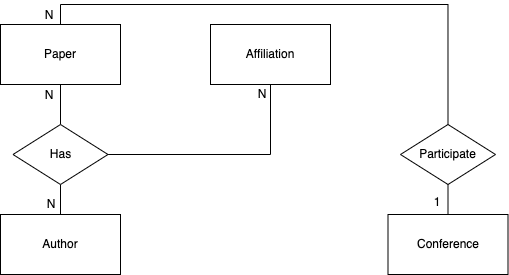
\includegraphics[width=0.8\linewidth]{er1.png}
    \caption{Modello ER del problema}
    \label{fig:er1}
\end{figure}

\chapter{Implementazione}

\section{Descrizione del progetto}
\label{descrizione_progetto}

% \todo{Una descrizione del progetto, con la separazione in fasi}
Il progetto si pone l'obiettivo di raccogliere una quantità rappresentativa
di paper, autori e conferenze degli ultimi anni al fine di derivare alcune
correlazioni fra le principali metriche, quali l'H-index, la qualità delle
conferenze ed il numero delle citazioni.

Il lavoro si suddivide principalmente nelle seguenti fasi:
\begin{enumerate}
  \item Modellazione dei dati inerenti al problema;
  \item Raccolta e organizzazione dei dati da varie fonti, quali Scopus e GGS;
  \item Integrazione dei dati in un unico modello al fine di creare un database unificato;
  \item Sviluppo di un'applicazione web in Django per la visualizzazione delle varie metriche.
\end{enumerate}

Oltre agli indici direttamente disponibili (e.g., H-index, citazioni, qualità
delle conferenze), sono state derivate alcune metriche per via campionaria.
Tra le principali analizzate vi sono:
\begin{itemize}
  \item La distribuzione della qualità delle conferenze analizzate;
  \item La distribuzione degli H-index degli autori;
  \item La distribuzione della qualità dei lavori per un certo autore;
  \item La correlazione tra qualità delle conferenze e distribuzione del numero delle citazioni dei paper;
  \item La correlazione tra la qualità di una conferenza e la distribuzione degli H-index degli autori coinvolti.
\end{itemize}
\todo{Vedere di aggiungerne altre}

%%%% STRUMENTI %%%%%
\section{Strumenti}

I dati che sono stati analizzati in questo progetto di tesi sono stati scaricati
dal database di Scopus utilizzando le API che il sito mette a disposizione.

Per implementare la dashboard e le varie pagine che mostrano i risultati delle
interrogazioni è utilizzato Python come linguaggio di programmazione, il
framework Django e SQLite come database.

%%%% SCOPUS API %%%%%
\subsection{Scopus API}

Scopus permette di accedere a circa 78 milioni di articoli, riviste
scientifiche, libri e pubblicazioni. Le API di Scopus permettono di visualizzare
abstract e dati riguardanti il numero di citazioni di tutte le riviste
accademiche indicizzate da Scopus.

Sono disponibili due modi di utilizzo delle API di Scopus: commerciale e
non commerciale. Per questa tesi sono state utilizzate le API a uso non
commerciale, disponibili gratuitamente per lavori senza scopo di lucro.
Utilizzando le API di Scopus si ha accesso diretto ai dati di Scopus in tempo
reale. Le \textit{API responses} includono link a risorse collegate, rendendo
la navigazione più semplice e la documentazione consente di visualizzare in
anteprima la richiesta e la risposta della API in modo interattivo. Inoltre
l'architettura RESTful permette di avere vantaggi di scalabilità, portabilità
e affidabilità.
Tali API risultano però sottoposte ad alcuni limiti, in quanto sono accessibili
solo da reti di atenei riconosciute da Scopus ed implementano rate limiting\footnote{\url{https://dev.elsevier.com/api_key_settings.html}}.

Una categoria di API importante è rappresentata dalla \textit{Scopus Search}~\cite{scopussearch}.
Essa può essere usata per accedere a dati riguardanti
paper, con relativi autori ed atenei. Ogni risultato fornito è collegato ad un
abstract e tramite link al resto del testo dell'articolo.
Questa API utilizza la sintassi booleana che consente agli utenti di combinare
parole chiave attraverso gli operatori \texttt{AND}, \texttt{OR} e \texttt{NOT},
per poter produrre risultati  più rilevanti. La ricerca booleana viene inviata
tramite il parametro \textit{query} della \textit{query string} e il contenuto
della ricerca inviata deve essere  codificato nell'URL.

\subsection{pybliometrics}\label{sec:pybliometrics}

\texttt{pybliometrics}~\cite{pybliometrics} è una libreria di Python che serve per estrarre e memorizzare nella cache i dati dal database Scopus.
Essa fornisce un insieme di classi che forniscono un'astrazione dalle chiamate
API di Scopus. Tali classi sono:
\begin{itemize}
	\item \texttt{AbstractRetrieval}: implementa l'API Abstract Retrieval di
	Scopus che consente di estrarre informazioni riguardo gli articoli;
	\item \texttt{AffiliationRetrieval}: implementa l'API Affiliation Retrieval
	di Scopus che fornisce informazioni riguardo gli atenei registrati, come per
	esempio città, paese e membri;
	\item \texttt{AuthorRetrieval}: implementa l'API Author Retrieval di Scopus
	che contiene tutte le informazioni riguardanti un autore;
	\item \texttt{ScopusSearch} implementa l'API di ricerca di Scopus, esegue una
	query per cercare documenti e quindi recupera i record della query.
\end {itemize}

Un esempio d'uso della API, preso da~\cite{pybliometrics}, è dato dal
Listing~\ref{lst:pybliometrics-example}.

\begin{lstlisting}[language=Python, caption=Esempio d'uso di \texttt{pybliometrics}, label=lst:pybliometrics-example]
from pybliometrics.scopus import AbstractRetrieval, AuthorRetrieval, AffiliationRetrieval

ab = AbstractRetrieval("10.1016/j.softx.2019.100263")

print(ab.title) # 'pybliometrics: Scriptable ...'
print(ab.authors) # > [Author(...), Author(...)]

au1 = AuthorRetrieval(ab.authors[0].auid)
au2 = AuthorRetrieval(ab.authors[1].auid)

print(au1.affiliation_current) # [Affiliation(...)]
print(au2.h_index) # 34

aff1 = AffiliationRetrieval(au1.affiliation_current[0].id)

print(aff1.author_count) # 98
\end{lstlisting}

\subsection{matplotlib}

\texttt{matplotlib}~\cite{matplotlib} è una libreria Python per la creazione
di grafi e visualizzazioni di dati in Python. In questo progetto la libreria
è stata usata per la creazione dei grafici rappresentanti metriche aggregate,
come ad esempio la distribuzione delle conferenze secondo il loro rating, 
al fine di semplificare la fruizione dei vari indici.

Inoltre, la libreria permette l'export delle visualizzazioni in vari formati,
come PNG, JPEG e PDF, anche integrabili direttamente in risposte a chiamate HTTP.
Fornisce inoltre la possibilità di creare visualizzazioni interattive, seppur
non usata in questo progetto di tesi.

L'interfaccia esposta da \texttt{matplotlib} è stata creata appositamente per
essere utilizzabile anche da persone con esperienza pregressa del linguaggio
Matlab, in quanto è molto simile al parco di funzioni fornite da quest'ultimo
per la creazione di grafi. Non solo, anche lo stile grafico predefinito è
ispirato da quello dato da Matlab.

Nel Listing~\ref{lst:matplotlib-example} si può vedere un esempio d'uso per
la creazione di un grafico a barre.

\begin{lstlisting}[float, language=Python, caption=Esempio d'uso di \texttt{matplotlib}, label=lst:matplotlib-example]
import matplotlib.pyplot as plt

xs = ['A++', 'A+', ...]
ys = [10, 20, ...]

plt.figure()
plt.title('Distribuzione del rating delle conferenze')
plt.bar(xs, ys)
plt.xlabel('Rating della conferenza')
plt.ylabel('Numero conferenze')
plt.show()
\end{lstlisting}


%%%% DJANGO %%%%%
\subsection{Django}\label{sec:django}

Django~\cite{django} è un framework web open source scritto in Python. È
un framework ``batteries included'', ovvero tenta di fornire più strumenti
possibile per ridurre sia la quantità di codice da scrivere sia la sua
complessità.

Django si basa sull'architettura \textit{Model, View, Template}, basata sulla più
classica MVC. Essa propone tre diverse entità per la gestione dei dati e dell'interazione
con l'utente, che sono:
\begin{itemize}
	\item \textit{Model}, la descrizione dei dati tramite una classe Python;
	\item \textit{View}, un sistema che processa le richieste degli utenti e
	definisce che dati devono essere presentati in risposta;
	\item \textit{Template}, un template HTML con un proprio linguaggio di templating
	chiamato DTL (Django Template Language) che definisce la rappresentazione
	grafica dei dati.
\end{itemize}
In questa categorizzazione, la \textit{View} di MVT corrisponde al \textit{Controller}
di MVC, mentre il \textit{Template} di MVT corrisponde alla \textit{View} di MVC.

\begin{lstlisting}[language=Python, caption=La classe \texttt{Author}, label=lst:author]
from django.db import models

class Author(models.Model):
    surname = models.CharField(max_length=200)
    name = models.CharField(max_length=200)
    citation_count = models.IntegerField()
    cited_by_count = models.IntegerField()
    h_index = models.IntegerField()
\end{lstlisting}

Django fornisce un ORM (\textit{Object-Relational Mapping}) tramite la
rappresentazione di tabelle con delle classi che derivano dalla classe
predefinita \texttt{Model}, come mostrato nel Listing~\ref{lst:author}. In
tal modo, è possibile interagire con degli oggetti Python, del tutto simili
alle classi, astraendo completamente dalla tecnologia di database utilizzata.
Infatti, con Django è possibile utilizzare diversi DBMS~\cite{djangoDBMS}, tra cui PostgreSQL,
MariaDB, MySQL e SQLite. Quest'ultimo è stato scelto per essere usato in questo
progetto di tesi, in quanto la semplicità e la facilità di setup sono risultate
fondamentali per velocizzare la realizzazione di prototipi.

Le \textit{View} di Django possono essere rappresentate da varie entità nel codice,
ma i modi principali sono le \textit{view generiche} tramite classi fornite dal framework
stesso e delle semplici \textit{funzioni} che lavorano su un parametro rappresentante
la richiesta effettuata dall'utente. Come esempio, nel Listing~\ref{lst:view-author-info}
è rappresentata una view che ottiene le informazioni di un autore specifico,
come salvate su database, aggiungendo inoltre una classificazione in base al
rating delle conferenze a cui ha partecipato.

\begin{lstlisting}[language=Python,caption=La view \texttt{author\_info},label=lst:view-author-info]
def author_info(request, author_id):
    author = get_object_or_404(Author, pk=author_id)
    num_confs = {}

    for pub in author.publication_set.all():
        rating = pub.paper.conference.ggs_rating
        if rating in num_confs:
            num_confs[rating] += 1
        else:
            num_confs[rating] = 1

    return render(request,
                  "author_info.html",
                  {"author": author, "num_confs": num_confs})
\end{lstlisting}

Infine, un \textit{Template} di Django è semplicemente un file HTML che
viene interpretato come codice DTL al momento della costruzione della risposta
inviata dal server al client che ha effettuato la richiesta. Un esempio di tale
template è visibile nel Listing~\ref{lst:django-template}.

\begin{lstlisting}[language=HTML, caption=Template per l'elenco delle conferenze,label=lst:django-template]



Conferences - Produzione Scientifica



<h1>List of Conferences</h1>

<img src="" />

<table>
  <thead>
    <tr>
      <th>Name</th>
      <th>Acronym</th>
      <th>Rating</th>
    </tr>
  </thead>
  <tbody>
    
    <tr>
      <td>
        <a href="">{{ conference.name }}</a>
      </td>
      <td>{{ conference.acronym }}</td>
      <td>{{ conference.ggs_rating }}</td>
    </tr>
    
  </tbody>
</table>

\end{lstlisting}

Django offre anche la possibilità di avere più di una \textit{app} su uno stesso
server web, ciascuna con le proprie views, i propri template ed il proprio
database. In questo modo, è possibile separare la configurazione generica del
server gestito da Django da varie applicazioni che girano su di esso.
Per questo progetto, la creazione di una singola app è più che sufficiente.

Django associa ad ogni possibile \textit{path} (o URL) di una richiesta HTTP
una certa view. Quando una richiesta HTTP viene inviata dal client verso il
server gestito da Django, quest'ultimo effettua una ricerca fra i propri path
definiti ed inoltra la richiesta, trasformata in un oggetto Python, alla
\textit{view} che si occupa della sua gestione.
Tale view può eseguire qualsiasi azione desiderata, come aggiorare il database o
leggere dati, anche differenziando in base al metodo HTTP usato dalla richiesta.
Una volta terminato però il lavoro necessario, la view è costretta a ritornare
una risposta al client, sia essa positiva o negativa, che la mostrerà all'utente
tramite un browser o qualsiasi altro tool usato.

\section{Ottenimento dei dati}

Come già anticipato in Sezione~\ref{sec:scopus}, la maggior parte dei dati è
stata presa da Scopus. In particolare, Scopus ha fornito i dati di circa 80000
papers negli ultimi 4 anni, con i relativi autori ed affiliazioni.
Per le conferenze, non fornendo Scopus informazioni se non nome ed acronimo
delle conferenze, si è fatto uso dei dati indicizzati da GII-GRIN-SCIE~\cite{giigrinscie} (GGS).

Per il download dei dati da Scopus, si è usato \texttt{pybliometrics}
(Sezione~\ref{sec:pybliometrics}) per lo sviluppo di script custom orientati
al download di grandi quantità di dati in modo automatico facendo uso delle
API fornite da Scopus.

Per quanto riguarda le conferenze, invece, i nomi delle conferenze forniti da
GGS non concordano in pieno con quelli presenti su Scopus. A questo fine,
si è manualmente proceduto all'analisi delle conferenze ottenute ed al loro
inserimento all'interno del database del progetto.
Al fine di semplificare e velocizzare il processo, si è fatto uso della
\textit{distanza di Levenshtein} per confrontare i nomi dati dalle due fonti.
La priorità è stata comunque data agli acronimi rispetto ai nomi interi.

\subsection{Distanza di Levenshtein}

L'algoritmo di Levenshtein, introdotta per la prima volta nel
1965~\cite{levenshtein1966} calcola la somiglianza tra due stringhe diverse.
Date due stringhe $a$ e $b$, l'algoritmo misura il numero di modifiche
elementari necessarie per trasformare la stringa $a$ nella stringa $b$.
Tra le operazioni elementari si hanno eliminazione di un carattere,
sostituzione di un carattere con un altro, inserimento di un nuovo carattere.
Più precisamente, definite $a$ e $b$ due stringhe, $|a|$ la lunghezza di una
stringa, la distanza di Levenshtein è definita come
\begin{equation*}
  \text{lev}(a, b) =
  \begin{cases}
    |a| & \text{se } |b| = 0 \\
    |b| & \text{se } |a| = 0 \\
    \text{lev}(\text{tail}(a), b) & \text{se } a_0 = b_0 \\
    1 + \min\begin{cases}
      \text{lev}(\text{tail}(a), b) \\
      \text{lev}(a, \text{tail}(b)) \\
      \text{lev}(\text{tail}(a), \text{tail}(b)) \\
    \end{cases}
    & \text{altrimenti}
  \end{cases}
\end{equation*}
%
Dove $\text{tail}$ rappresenta la coda di una lista, i.e., se $a_i$ è il
carattere in posizione $i$, allora data la stringa $a = a_0a_1\cdots a_n$ si ha
che $\text{tail}(a) = a_1\cdots a_n$.
Nell'implementazione è stata usata la libreria
\texttt{python-Levenshtein}~\cite{pythonLevenshtein}.

Al fine di dimostrare brevemente il ragionamento intrapreso, si prendano come
esempio le due stringhe \texttt{kitten} e \texttt{sitting}. In tal caso, si
ha che $\text{lev}(\text{kitten}, \texttt{sitting}) = 3$. Infatti, la seconda
stringa si può ottenere dalla prima effettuando le sostituzioni $k \to s$
e $e \to i$, con l'aggiunta finale della lettera \textit{g}.
Di conseguenza, essendo le modifiche elementari pari in numero a 3, esso è
anche il valore assunto dalla distanza di Levenshtein.

%%% DOWNOLAD DEI DATI %%%%
\section{Descrizione dei dati}\label{sec:descrizionedati}

In Figura \ref{fig:logico} è visibile lo schema logico, rappresentante
le tabelle presenti direttamente nel database, coi relativi attributi e chiavi
esterne. Notare la presenza della tabella \textit{Publication}, in sostituzione
alla relazione tripla nominata in Sezione~\ref{sec:modellizzazioni}.

Al fine di identificare univocamente i dati, si è fatto uso dei campi
identificativi forniti direttamente dal database di Scopus. Questo per evitare
ambiguità con un'eventuale generazione automatica a partire dai dati,
soprattutto in caso di omonimie.

\begin{figure}
  \centering
  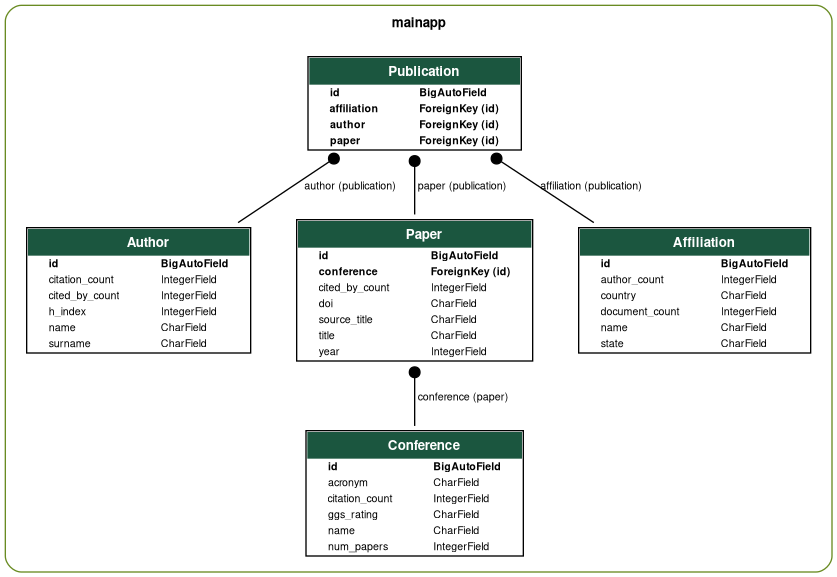
\includegraphics[width=0.8\linewidth]{logico.png}
  \caption{Schema logico del problema}
  \label{fig:logico}
\end{figure}

\subsection{Affiliation}

Un'affiliazione rappresenta un'università, e per ogni singola entry si ha
interesse a mantenere i seguenti campi:

\begin{itemize}
  \item \texttt{aff\_id}, l'identificativo dell'università;
  \item \texttt{affiliation\_name}, nome dell'università;
  \item \texttt{state} e \texttt{country}, contenenti informazioni riguardanti la posizione geografica dell'università;
  \item \texttt{author\_count}, numero di autori associati all'università;
  \item \texttt{document\_count}, numero di documenti per l'università.
\end{itemize}

\subsection{Author}
Un autore è rappresentato dai seguenti campi:
\begin{itemize}
  \item \texttt{author\_id};
  \item dati per il nominativo, ovvero \texttt{surname} e \texttt{name};
  \item \texttt{citation\_count}, numero totale di elementi citati;
  \item \texttt{cited\_by\_count}, numero totale di autori citanti;
  \item \texttt{h\_index}, h-index dell'autore.
\end{itemize}

\subsection{Conference}

Di una conferenza ci interessa mantenere i seguenti campi:
\begin{itemize}
  \item \texttt{title}, nome della conferenza;
  \item \texttt{acronym};
  \item \texttt{ggs\_rating}, il rate come definito da GGS;
  \item \texttt{num\_papers}, numero di paper accettati dalla conferenza;
  \item \texttt{citation\_count}, numero di citazioni totali di tutti i paper della conferenza.
\end{itemize}

\subsection{Paper}

Un paper viene rappresentato dai seguenti dati:

\begin{itemize}
  \item \texttt{id};
  \item \texttt{authors}, lista di autori del paper (rappresentati dai relativi identificativi);
  \item \texttt{title};
  \item \texttt{year};
  \item \texttt{conference}, la conferenza a cui è stato presentato;
  \item \texttt{cited\_by\_count}, il numero di citazioni;
  \item \texttt{doi}, il suo identificativo DOI.
\end{itemize}

% \section{Implementazione di views e metriche}

\section{Applicazione web}

L'applicazione web realizzata in questo progetto di tesi offre la funzionalità
di accesso semplificato ai dati ottenuti e, più importantemente, di visualizzazione
delle varie analisi metriche ottenute.

\subsection{Struttura dei file}

% \todo{Descrivere la separazione data da Django nei file e nel codice}

La struttura di file e directory di un'applicazione web scritta con Django 
segue una forma fissa, definita dal framework, che permette l'organizzazione
delle varie parti di codice in base al loro ruolo all'interno dell'architettura.
Le principali sezioni in questo progetto sono date da:
\begin{itemize}
  \item La directory \texttt{mainapp}, che contiene il codice della \textit{app}
        principale di Django;
  \item Il file \texttt{manage.py}, che offre un'interfaccia da riga di comando
        per la gestione di migrazioni sul database, l'avvio e l'arresto di server
        web locali, e simili operazioni di gestione del progetto;
  \item Una directory \texttt{prodsc} per i file usati da Django nella configurazione
        dell'intera applicazione web.
\end{itemize}

A sua volta, la cartella \texttt{mainapp} contiene i seguenti:
\begin{itemize}
  \item \texttt{admin.py}, che contiene le definizioni base per permettere l'uso
        della console di amministrazione offerta da Django;
  \item \texttt{apps.py}, per la configurazione di eventuali app interne a \texttt{mainapp};
  \item \texttt{forms.py}, la definizione del form di upload dei dati, usato per la
        semplificazione della conversione dei dati CSV ottenuti dalle API per
        poter essere inseriti in database;
  \item \texttt{images.py}, che definisce tutte le view per la generazione di
        grafici di metriche tramite \texttt{matplotlib};
  \item \texttt{migrations}, una cartella per le varie migrazioni del database SQLite;
  \item \texttt{models.py}, il modulo che definisce le varie classi dei modelli
        come descritto in Sezione~\ref{sec:django};
  \item \texttt{static}, per file statici come CSS e JavaScript;
  \item \texttt{templates}, directory contenente i diversi template usati dalle view;
  \item \texttt{urls.py}, che definisce gli endpoint accettati da Django e quale
        view è responsabile per la gestione di ciascuno di essi;
  \item Ed infine \texttt{views.py}, le diverse views per la visualizzazione
        dei vari dati utilizzati.
\end{itemize}




%% Dashboard

\subsection{Dashboard}
Di seguito è descritta come è stata realizzata la dashboard per la visualizzazione dei dati e delle metriche realizzate.

Come stile delle pagine web viene utilizzato \textit{Bootstrap}, un framework per lo sviluppo front-end. 
Nel file \texttt{base.html}, contenuto nella directory \texttt{templates}, è contenuto il codice dello stile, che presenta una barra laterale per la navigazione del sito, come visibile nel Listing~\ref{lst:base_html}.

Come visibile dal codice, in Django si utilizza il tag \texttt{\{\% block \%\}} per definire un blocco che può essere sovrascritto dai modelli che ne derivano. In questo codice viene definito il blocco del modello base, per ogni pagina verrà poi definito un blocco figlio con contenuti diversi. I blocchi utilizzati sono:


\begin{itemize}
  \item \texttt{\{\% block title \%\}}: per il titolo della pagina web;
  \item \texttt{\{\% url \%}\}: per l'url della pagina collegata;
  \item \texttt{\{\% block content \%}\}: per il contenuto della pagina.
\end{itemize}

\begin{lstlisting}[language=html, caption=Estratto di \texttt{template/base.html}, label=lst:base_html]
<html>
<head>
  <title>Produzione Scientifica</title>

  
  <link rel="stylesheet" type="text/css" href="" />
  <link rel="stylesheet" type="text/css" href="" />
</head>

<body>
  <div id="wrapper">
    <ul class="navbar-nav bg-gradient-primary sidebar sidebar-dark accordion" id="accordionSidebar">

      <!-- Sidebar - Brand -->
      <a class="sidebar-brand d-flex align-items-center justify-content-center" href="">
        <div class="sidebar-brand-text mx-3">Produzione scientifica</div>
      </a>
      <!-- Divider -->
      <hr class="sidebar-divider my-0">
      <li class="nav-item">
        <a class="nav-link" href="">Affiliations</a>
      </li>
      ...
    </ul>
    <!-- Content wrapper -->
    <div id="content-wrapper" class="p-5 d-flex flex-column">
    </div>
  </div>

</body>
</html>
\end{lstlisting}

Nella Figura \ref{fig:homepage} è mostrata l'hompage del sito che contiene ... 
\todo{Descrivere cosa si visualizza nella prima pagina}

\begin{figure}
  \centering
  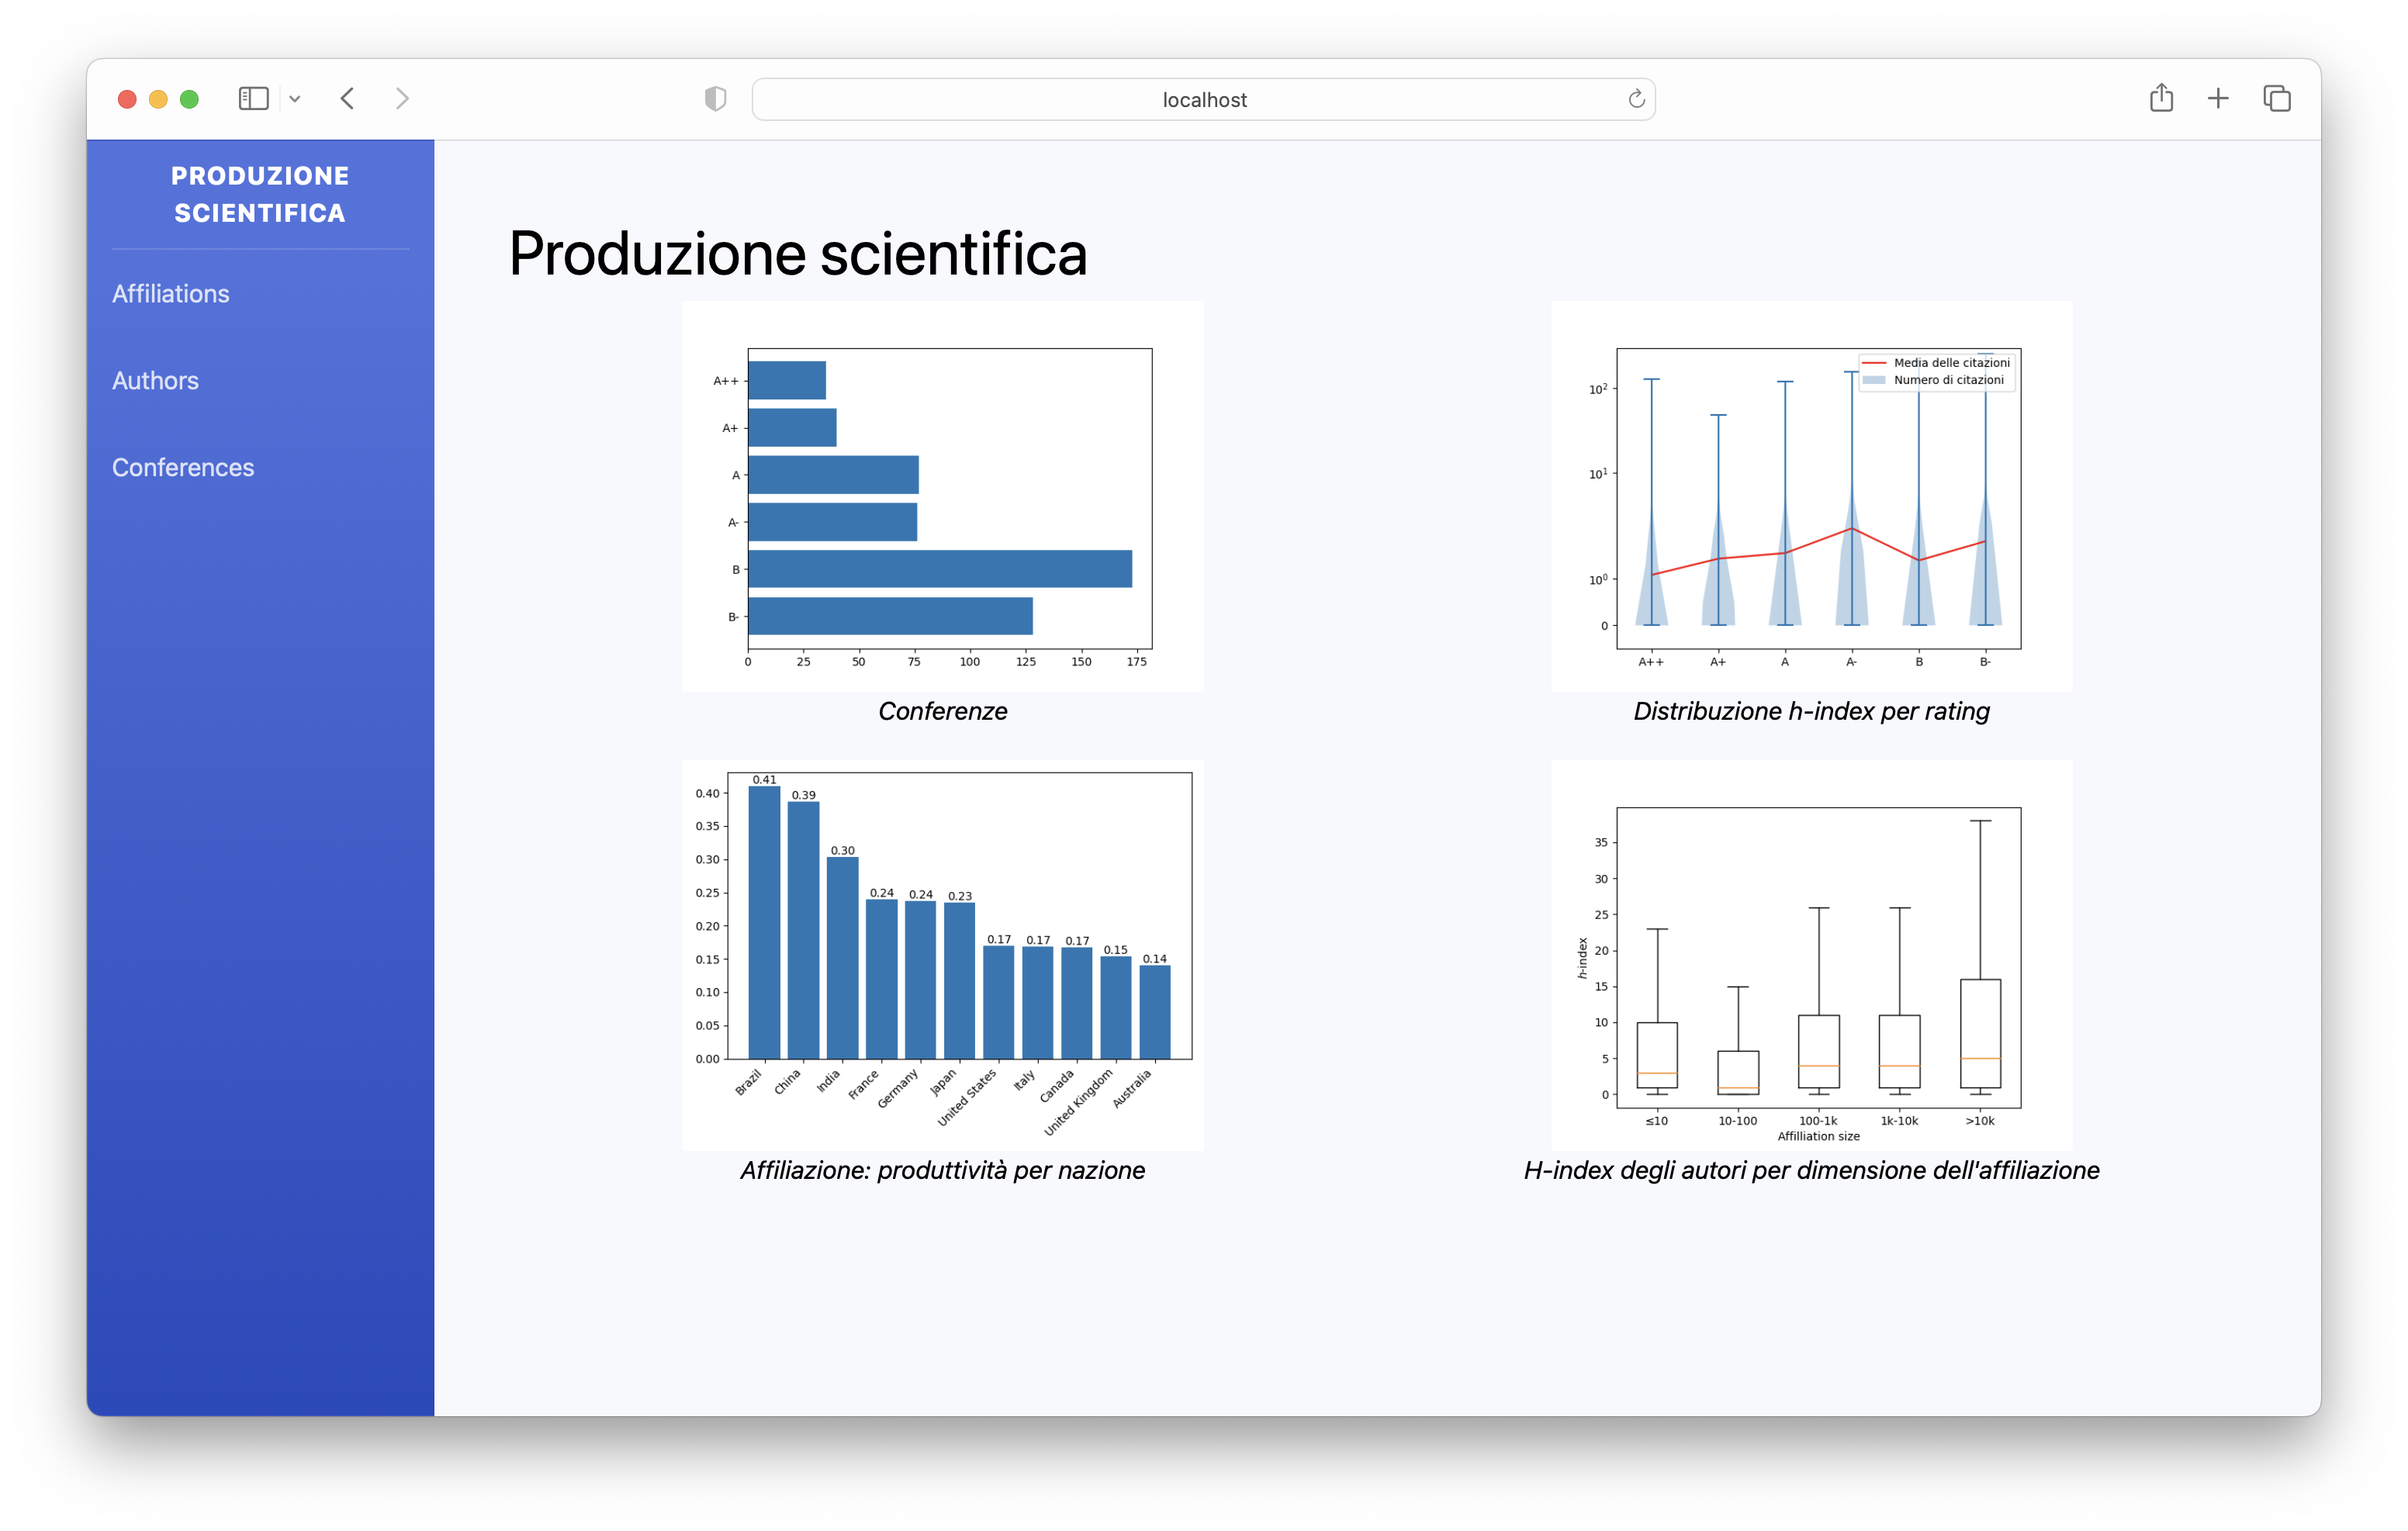
\includegraphics[width=0.8\linewidth]{homepage.png}
  \caption{Modello ER del problema}
  \label{fig:homepage}
\end{figure}

\subsubsection{Visualizzazione dei dati del database}
Per le entità Affiliation, Author e Conference sono state dedicate delle pagine per la visualizzazione dei dati presenti nel database.

Prendendo per esempio le Affiliation, nel Listing \ref{lst:affiliation_html} è mostrato il codice per la visualizzazione della tabella dei dati contenuti nel database. 


\begin{lstlisting}[language=html, caption=Estratto di \texttt{template/affiliation.html}, label=lst:affiliation_html]
  


Affiliations - Produzione Scientifica



<h1>List of affiliations</h1>

<table>
  <thead>
    <tr>
      <th>Name</th>
      <th>Country</th>
      <th>Num. of Authors</th>
      <th>Average H-Index</th>
    </tr>
  </thead>
  <tbody>
    
    <tr>
      <td>
        {{ a.name }}
      </td>
      <td>{{ a.country }}</td>
      <td>{{ a.author_count }}</td>
      <td>{{ h_index }}</td>
    </tr>
    
  </tbody>
</table>

  
\end{lstlisting}

Nella sezione successiva invece verrà introdotto il codice per il calcolo delle metriche.

%% Calcolo delle metriche

\subsection{Calcolo delle metriche}

Le metriche sono calcolate tramite codice Python scritto ad-hoc per ogni
caso, usando i dati salvati nel database descritto nelle sezioni precedenti.
Per comodità ed organizzazione, per ogni metrica che ha una rappresentazione
tramite immagine è presente una view in \texttt{mainapp/images.py}.

Tali immagini sono ottenute tramite \texttt{matplotlib}. Dove necessario,
\texttt{pandas} e \texttt{numpy} offrono delle capacità di manipolazione dati
più avanzate di quanto disponibile direttamente dall'ORM di Django.

Come esempio, prendiamo la distribuzione delle conferenze usate in questo
progetto, analizzata ulteriormente in Sezione~\ref{sec:distrib-conferenze},
al fine di illustrare la realizzazione di una semplice immagine.
Come si può vedere nel Listing~\ref{lst:distrib-conf}, l'immagine viene creata
tramite una view di Django. La differenza principale è data dalla creazione
di una \texttt{figure.Figure} tramite la libreria \texttt{matplotlib}.
Inoltre, la risposta ritornata dalla view ha un \texttt{Content-Type} pari a
\texttt{image/png}, cosicché il client non interpreti erronamente il contenuto
come testo o come HTML.

\begin{lstlisting}[language=Python, caption=Distribuzione delle conferenze, label=lst:distrib-conf]
import matplotlib.figure as figure

def create_image(fig):
    resp = HttpResponse(content_type="image/png")
    fig.savefig(resp)
    return resp

def conferences_distribution(request):
    ratings = list(reversed(["A++", "A+", "A", "A-", "B", "B-"]))  # I want A++ on top
    counts = [len(Conference.objects.filter(ggs_rating=rating)) for rating in ratings]

    f = figure.Figure()
    ax = f.add_subplot()

    ax.barh(ratings, counts)

    return create_image(f)
\end{lstlisting}

Successivamente, come ogni altra view, è necessario fornire un URL a cui
Django risponderà con l'immagine creata. Tale passo è visibile nel
Listing~\ref{lst:distrib-conf-urls}, che contiene un estratto del file
\texttt{mainapp/urls.py}.

\begin{lstlisting}[language=Python, caption=Estratto di \texttt{mainapp/urls.py}, label=lst:distrib-conf-urls]
from django.urls import path
from . import views, images

urlpatterns = [
    # ...
    path(
        "conferences/distribution.png",
        images.conferences_distribution,
        name="conferences_distribution.png",
    ),
    # ...
]
\end{lstlisting}

\chapter{Metriche}
In questo capitolo verranno descritte le metriche anticipate nella Sezione \ref{descrizione_progetto}, mostrando il relativo codice e i risultati ottenuti.


\chapter{Conclusioni}

\chapter*{Ringraziamenti}
In conclusione di questo elaborato, voglio ringraziare il mio relatore Stefano Paraboschi e il SecLab per avermi seguito nello sviluppo del progetto.

Ringrazio la mia famiglia e i miei amici per aver condiviso con me questi anni di università.

\nocite{*}
\printbibliography[heading=bibintoc]

\end{document}
